%  MDW Version 0.0  details here
\documentclass[12pt,oneside,doublespace,pdflatex]{amsart}
%%% Bibliography
%\usepackage[sort&compress]{harvard}   
\usepackage{natbib}
\usepackage{tikz}
\date{Amsterdam \today~version 0.01.}
%%% HEADERS & FOOTERS
\usepackage{fancyhdr}  
\usepackage{blindtext}
\pagestyle{fancy}  
\renewcommand{\headrulewidth}{0pt}  
%\lhead{ }\chead{Forecasting Conflict}\rhead{\today}
%\lfoot{\sc \tiny ISR}\cfoot{\thepage}\rfoot{\sc \tiny Submission}
\footskip=35pt
\parindent .49 in 
%\raggedright
\let\footnotesize\normalsize
\usepackage{geometry}
\geometry{verbose,tmargin=1in,bmargin=1in,lmargin=1in,rmargin=1in}
% Add some colors
\definecolor{green1}{RGB}{229,245,224}
\definecolor{green2}{RGB}{161,217,155}
\definecolor{green3}{RGB}{49,163,84}

\definecolor{blue1}{RGB}{239,237,245}
\definecolor{blue2}{RGB}{188,189,220}
\definecolor{blue3}{RGB}{117,107,177}


%\pdfpagewidth=8.5in % for pdflatex
%\pdfpageheight=11in % for pdflatex

%%% END Article customizations
%%% PACKAGES
%\usepackage{booktabs} % for much better looking tables
\usepackage{array} % for better arrays (eg matrices) in maths
\usepackage{paralist} % very flexible & customisable lists (eg. enumerate/itemize, etc.)
\usepackage{verbatim} % adds environment for commenting out blocks of text & for better verbatim
\usepackage{graphicx}
\usepackage{caption}
\usepackage{subcaption}
%\usepackage{subfigure}%
%\usepackage[usenames]{color}
%\usepackage{booktabs}
%\usepackage{dcolumn}
%\usepackage{tabularx}
%\newcolumntype{d}{D{.}{.}{-1}}
%\usepackage{hyperref}
%\usepackage{lscape}
%\input xy
%\xyoption {all}
%\usepackage{wrapfig}
%\usepackage{placeins}
\usepackage{xcolor}
%\usepackage{float}
\usepackage{amsfonts,amsmath,amssymb}
\usepackage{array,psfrag,tabularx,booktabs}
\usepackage{mparhack}
\usepackage{setspace}
\usepackage{natbib}
\usepackage{multicol}
\usepackage{endnotes}
\usepackage{dcolumn}
%\usepackage{hyperref}
\usepackage{url}
\usepackage{stmaryrd}
\setcitestyle{authordate,round,semicolon,aysep={,},yysep={,}}
\bibpunct[, ]{(}{)}{;}{a}{,}{,}
%\doublespacing
\graphicspath{{graphics/}}
\begin{document}

\title[Not Power]{Influence Networks in International Relations}

\author{Michael D. Ward}
%\thanks
\address{Michael D. Ward: Department of Political Science, Duke University, Durham, NC, USA, 27707\\}
\email{michael.d.ward@duke.edu}
 
\author{Peter D. Hoff}
%\thanks{}
\address{Peter D. Hoff: Department of Statistics, University of Washington, Seattle, WA, USA, 98195}
\email{pdhoff@u.washington.edu}

\author{Shahryar Minhas}
%\thanks{}
\address{Shahryar Minhas: Department of Political Science, Duke University, Durham, NC, USA, 27707\\}
\email{shahryar.minhas@duke.edu}

\begin{abstract} THIS ABSTRACT WILL DIE.
There is a long history of power in international relations and world politics. As early as 275 BCE, the writings attributed to Chanakya (also known as Kautilya) were influential in discussing power between states.  In historical Chinese writing power is rarely discussed, but may be assumed. During the 16th century in Europe, Machiavelli famously wrote what a prince had to do to maintain his power. But conceptual definitions and quantitative measurements are much more recent, and emanate from a European tradition.  We show that there is no widely agreed upon definition of power that can be used in a principled, empirical fashion.  All extant, empirical measures focus either on a) material capabilities or b) mystical properties. We propose a relational, network model of influence relationships among international actors and derive its properties. We demonstrate its descriptive benefits as well as illustrate how it may be used to improve empirical studies which aspire to study power.
\end{abstract}
 
\pagestyle{fancy} \chead{} \rhead{}
\lhead{Influence in International Relations} \cfoot{\arabic{page}} \rfoot{}

\maketitle

\begin{quote} {\em
I was able to have a very successful career in political science without ever using the word ``power.'' You should do the same.}  Heinz Eulau,  $\sim$ 1984
\end{quote}

\section{Introduction}
\vskip .3cm
According to standard historical accounts,
the reign of Henry VIII of England (1509--1549) was largely devoted to preserving the {\em balance of power} by preventing Spain and France from joining forces and ruling Europe and conquering England.\footnote{Though maybe it was simply chronic traumatic encephalopathy.}  Thus, in numerous accounts of world politics beginning with the 16th Century and continuing until the end of empire, Britain was considered to be the ``balancer'' in world politics. And for a large number of analysts,  world politics
was thought to be a system of state led politics in which power was balanced \citep{spykman:1942,gulick:1955}.\footnote{Thucydides used this concept in his explanation for the onset of the
Peloponnesian Wars.  See also the essay by \cite{hume:1742}.} This, of course, was a very specific reading of history, one that is wildly at odds with contemporary historical analysis.\footnote{Henry VIII and Cardinal Wolsley are now thought
to have been more tactical than strategic, and not really interested in balancing {\em per se}, but rather in protecting and in limited ways expanding England.  Even the Treaty of London was quickly abandoned and the Treaty of Bruges can be seen as pragmatic, not strategic. See \citet{raymond:2007} among others.  Most accounts of the balancing also fail to consider the role of the Holy Roman Empire as an actor in this play.}  However, the notion of the balance of power has survived to contemporary times and is well entrenched in the social sciences.\footnote{See \citet{zinnes:1967,dorussen:1999,fearon:1994,kadera:2001,moul:2005,nexon:2009,wolford:2015}, among a long list of others.} An early attempt to clarify the many different meanings of the concept of the balance is found in \citet{haas:1953}; however, the murkiness of this concept continues to this day.  A balance is a weighing, as in measurement, and requires some metric, however crude.  As yet, despite centuries of examining this question we have yet to arrive at an agreed to definition or metric of power.

Even apart from the concept of a balance, contemporary policy accounts often draw upon the concept of power, but rarely have a specific definition of what exactly this term refers to. Consider Angela Stent's recent analysis of what do do about Russia's military involvement in Syria 
\cite{stint:2016}. She notes
\begin{quote}
For all of Russia's domestic problems---a shrinking economy, a declining population, and high rates of capital flight and brain drain---it has projected a surprising amount of power not only in its neighborhood but also beyond. U.S. President Barack Obama may refer to Russia as a regional power, but Russia's military intervention in Syria demonstrates that it once again intends to be accepted as a global actor and play a part in every major international decision.
\end{quote}
But it is not clear exactly what is meant by Russia's power in this policy analysis by one of the leading scholars on Russian and Eastern European foreign policy. Is it the power to coerce Syria to ``stay the course'' against ISIS? Is the power to militarily defeat ISIS?  Is it the power to legitimize the Syrian government against it critics, internal and external? Is it simply the use of military force? Or, is it trying to recalibrate the balance of power so that Assad and his allies may prevail? In such policy analyses, power is often used variously to refer to influence, to victory in a conflict, to control over resources, and to status.  In many scholarly 
analyses power itself is a goal \citep{morgenthau:1948,waltz:1979}.  Often these meanings are woven together, somewhat selectively. 
\citet[page 24]{gilpin:1975} has suggested that the way in which political scientists define and deal with the concept of power is
an ``embarrassment.''  While pointing to many of these same issues, \citet{baldwin:1978} asserts
a widespread agreement on the necessity of using the concept of power to analyze international interactions. Both Gilpin and Baldwin suggest a relational approach to power as a compliment to the study of power as a material characteristic.
Yet, what this has mostly meant is direct comparison of the capability of one country with another, rather than an deeper consideration of the relational interpretation of power and strength.  
It has become a standard approach to use the ratio of capabilities for a measure of relative power in 
empirical studies 
\citep[among others]{slantchev:2004,reed:etal:2008,butler:gates:2009,gartzke:weisiger:2014,carter:poast:2015}.

Looking back, the first quantitative measurement of power was stimulated by the work of \cite{fucks:1965} which was quickly followed up on in \cite{morgenstern:1974}.  Perhaps this lead to an empirical assessment of power that was largely based on capabilities, and material.  Certainly the availability of quantitative data on material characteristics of states was to influence
greatly the scholarship in this area and many scholars were to rely on the Correlates of War's Composite Index of National Capabilities (CINC) measures as a way of assessing power \citep{singer:etal:1972}.\footnote{Version 4.0 of these data, 
through 2007, are available at \url{http://correlatesofwar.org/data-sets/national-material-capabilities}. See also \citet{park:ward:1988}.}  This pushed scholarly consideration of power into a capabilities direction, rather than a direction in which power was seen as relational.  These approaches have implicitly assumed that power is material 
{\em and} fungible. If China has more capabilities than India, it has more power. If India and Japan together have more capabilities than China, then they have more power. This kind of approach ignores the nuances of regional as well as global interactions, as well as ignoring the contexts in which states interact.  As such, it is easy to confound this understanding with simple examples. For example, since the US has more capabilities than North Korea, it has more power than North Korea and can prevent North Korea from doing something that it objects too, such as launching a satellite.\footnote{A kind of contrarian, network power was introduced in \cite{ward:house:1988,house:ward:1988} to capture the kind of power that rogue states may have.}

\section{Influence and Networks in International Relations}

A relational look a world affairs suggests, if not demands, a network perspective.  Fortunately in recent years there has been an increase in studies that examine the network of international relations.
Interestingly there was a brief period in the 1970s stimulated largely by
Johan Galtung's development of a structural theory of imperialism, which had crude networks, 
\citeyear{galtung:1971} in which there was considerable interests in networks as a way of understanding
the world system.  Early works include 
\cite{skjelsbaek:1972,chasedunn:rubinson:1977,bornschier:metal:1979,chirot:hall:1982}. These ideas largely grew into the
so-called world systems theory subfield of sociology, which thrives but is fairly isolated, even within sociology.

Fundamental work in physics energized the study of networks in the social world.  Following his dissertation on the topic,
Duncan Watts (with Steven Strogatz) introduced the idea of a small world \citep{watts:strogatz:1998,watts:2004a} which captured widespread attention. This work was further generalized in \citet{newman:etal:2001} which permitted
a wide array of distributional assumptions.  The network phenomenon was popularized by 
\citet{watts:2004}, \cite{christakis:fowler:2009}, and the explosive popularity of Facebook and Twitter.  In a short decade,
networks moved from being an arcane, academic topic, to something that was becoming part of contemporary culture.

These developments in physics and sociology coupled with advances in led scholars to begin using
modern approaches to networks to study world affairs.  \citet{ward:hoff:etal:2003} used latent network
models to study interactions among nations, groups within nations, and individuals, focusing especially on Central Asia, including Afghanistan and surrounding regions. The basic idea was to model the network dependencies directly but within a broader regression based framework. This was generalized and expanded in \citet{hoff:ward:2004} and applied to trade and conflict in \citep{ward:hoff:2007}. This latent approach--described in \citet{dorff:ward:2013}--was used to examine the Kantian piece \citep{ward:siverson:cao:2007}, policy networks \citep{cao:2009,cao:2010}, migration patterns \citep{breunig:cao:etal:2011}, international commerce \cite{ward:ahlquist:etal:2012},  and human rights \citep{greenhill:2015}, among other substantive issues.\footnote{See also the working paper by \citet{stewart:2014} for a discussion of factor models in the social sciences.}

At the same time, network studies of world affairs also followed a longer standing tradition which was established in sociology, based largely on the idea that you could calculate sufficient statistics for networks, and include them in simple logistic regression models \citep{frank:1971,besag:1977b}.  This simple approach was overturned by modern statistical techniques, which permitted a general approach to studying what became known and random Markov fields \citep{besag:1985,besag:clifford:1989}. But for many, this rested on using network characteristics in estimating regression models. The field known as {\em social network analysis} (SNA) developed and expanded these ideas.  SNA has a long tradition going back at least to the iconoclastic efforts of Joseph Moreno \citeyear{moreno:1934} to disprove Freudian approaches to psychological analysis.  A good history of the SNA movement in sociology and beyond can be found in \citet{freeman:2004}.\footnote{See also \cite{white:1963,granovetter:1973,white:boorman:breiger:1976,freeman:1978,burt:1982,freeman:2000} for seminal contributions to the methodology.}

As SNA is applied in world affairs, a non-network model---typically a standard country-year, dyad, panel---is estimated, but measurements of network characteristics of countries or dyads included as covariates.  Among the first to bring SNA to international relations were Emily Hafner-Burton \citep{hafner-burton:2006,hafner-burton:kahler:etal:2009} and Zeev Maoz \citep{maoz:2006a,maoz:terris:etal:2007,maoz:2010}.  This approach became quite popular in political science broadly
\citep{ward:stovel:etal:2011} and in the study of world affairs, as well 
\citep[for example]{lagazio:russett:2004,warren:2010,maoz2012special,kinne:2012,kinne:2013,kinne:2014,murdie:2014,haim:2016,wilson:etal:2016,warren:2016,ward:dorussen:2016,boehmelt:2016,kinne:2016,lupu:poast:2016,gartzke:westerwinter:2016,maoz:joyce:2016}.  The SNA model has focused largely on binary ties among nodes or countries. But this has been recently addressed by innovative work in two domains.  Skyler Cranmer and Bruce Desmarais have focused on making the so-called exponential random graph model (ERGM) more user friendly and conceptually flexible \citep{cranmer:desmarais:2011,cranmer:desmarais:etal:2012,desmarais:cranmer:2012,cranmer:desmarais:2015c}.  At the same time, Tom AB Snijders and his colleagues have focused on developing simulation techniques for modeling dynamic networks of strategically oriented actors 
\citep{snijders:etal:2010,snijders:2014,amati:2015}.  This latter approach has been recently used to study some aspects of world politics \citep{manger:pickup:2016}.\footnote{An as yet more minor, but promising thrust is the study of networks on games \citep{metternich:dorff:etal:2013,gallop:2015,gallop:2016,chyzh:2016,larson:2016}.}

\section*{Influence}

To study networks requires a great deal of data. Fortunately, we are awash in data.  But the tradition of using data on the events among and within nations has a longer history than contemporary data science. As part of the studies of the cables released after the first world war, Robert C. North and colleagues developed a method of content analyzing text that serves as the foundation for modern event data repositories \citep{north:etal:1963}. This work lead to fundamental discoveries about the ebb and flow of perceptions during the crises leading up to the outbreak of military hostilities in 1914 \citep{north:1967}.
The basic event data framework essentially developed initially by hand and encoded newspaper stories--typically fro the New York Times---about
world affairs in which an actor or initiator--typically on behalf of a country--under took some form of action, toward a target. Actions ranged from cooperative to conflictual, and could be verbal interactions or physical ones.  As part of his Dimensions of Nations project, Rummel first published summaries of the events within and between 89 nations over the period from 1955-1960  (\citeyear{rummel:1963}) and followed that with more detailed, factor analyses of these and other data (\citeyear{rummel:1976a}).

Charles McClelland \citep{mcclelland:hoggard:1969} created what became the backbone of modern event data systems when he designed the World Event Interaction Survey, also known as WEIS. There were almst two dozen 
low level categories which could describe an action between an initiating country and the actions recipient. These categories
ranged from cooperative actions such as yield and approve toward more conflictual ones such as threaten or force.\footnote{The categories are: 
Yield,
Comment,
Consult,
Approve,
Promise,
Grant,
Reward,
Agree,
Request,
Propose,
Reject,
Accuse,
Protest,
Deny,
Demand,
Warn,
Threaten,
Demonstrate,
Reduce relations,
Expel,
Seize, and
Force. }

Edward Azar (\citeyear{azar:1980}) expanded the WEIS framework and data sources and created the COPDAB, though these were still hand coded. Others, including 
Charles Hermann (\citeyear{hermann:etal:1973}), developed more focused efforts such as the
CREON database focusing on crisis events among a random set of countries.
But the creation of machine coded event data completely changed the scope and availability of detailed data that could
be used to quantitatively study the ebb and flow of world politics.  Working with early desktop computers, Philip Schrodt and colleagues began to create new data using automated methods, instead of using human coders. The earliest efforts expanded the WEIS categories to encompass mediation as well as confrontation \citep{schrodt:1994,gerner:etal:1994,schrodt:1997,gerner:schrodt:yilmaz:abujabr:2002}.
The so-called CAMEO ontology includes over 200 categories of verbs, classified into $20$ high level categories, as shown
in Table~\ref{tab:cameo}. The CAMEO approach was widely adopted and adapted by 
\citet{bond:etal:2003},
\citet{king:lowe:2003}, and others.\footnote{See also the descriptions by
\citet{schrodt:vanbrackle:2013} and \citet{
schrodt:2013}.}

\begin{table}
\caption{The CAMEO Event Categories (verbs). \label{tab:cameo}}
\begin{center}
\begin{tabular}{ll}
Comment & Disapprove \\
Consult & Reject \\
Approve & Threaten \\
Improve Relations& Protest \\
Request & Military Posture \\
Agree & Reduce Relations \\
Provide Aid & Structural Violence \\
Yield & Unconventional Violence \\
Investigate & Conventional Force \\
Demand & Unconventional Warfare \\
\end{tabular}
\end{center}
\end{table}


The so-called KEDS (now CEDS) database was widely used, and the ontology was adapted by a DARPA project on 
early warning called ICEWS.  ICEWS took the CAMEO ontology and expanded the codebook substantially, and changed the way in which events were coded. The early approaches had used a bag-of-words approach, but the ICEWS team adopted
an approach based on word-graphs and natural language processing \citep{boschee:natarajan:etal:2013}. This was compared to gold-standard, hand coded events and shown to improve accuracy considerably (beyond King and Lowe (2003)). This framework was used to encode (to date) over 30 million events for most countries in the world using a data corpus taken from Factiva and other sources that approaches 300 individual, electronic news sources. An archive of these data is publicly available at \url{https://dataverse.harvard.edu/dataverse/icews}; currently these data have been downloaded over seven thousand times. See also 
\citet{icews:2015:aggregations,icews:2015:data,ramshaw:etal:2011}.  In spite, or because of, the elaborate coding framework that is established for over 200 nuanced events, along with detailed dictionaries of actors for each country, in total number in the thousands, it is possible to distill these many different kinds of events into four types, which are commonly known as {\em quad code} variables: material conflict, verbal conflict, material cooperation, and verbal cooperation.

These ICEWS event data are the most extensive event database ever assembled. They include $22,669,257$ events since 1 January 2001 drawn from $38,309,404$ stories. In the year 2014 there are $871,555$ events.


\begin{figure}[h!]\caption{\it Cooperative Verbal Interaction Network, 2014 ($\sim$ 800K events). \label{fig:hairball}}
   \centering 
    \begin{subfigure}[b]{.69\textwidth}
        \includegraphics[width=.69\textwidth]{verbCoop2014.pdf}
        \caption{\it Cooperative Network 2014}
    \end{subfigure}
    \begin{subfigure}[b]{.3\textwidth}
        \includegraphics[width=\textwidth]{legend.pdf}
        \caption{\it Legend}
    \end{subfigure}
\end{figure}
Figure~\ref{fig:hairball} illustrates the network of cooperative interactions among over $200$ contemporary
countries for the calendar year 2014, based on the ICEWS event data.  This typical network ``hairball'' doesn't revel much
except that there are lots of linkages. Indeed, the modal number of events in 2014 is $550$, with a maximum of
over $50,000$.  Yet the average path length is $1.8$, but the reciprocity is fairly high ($0.88$) and
the transitivity is $0.57$, which is fairly strong. European and North American countries are grouped together with lots of
linkages, while the Latin American and African countries also form apparent clusters.  Despite the difficulty of visually
identifying what is going on in this network hairball, network techniques can tell us a great deal of information.  Among the low hanging network fruit typically employed in social network analysis are a variety of concepts that fall out of standard
country-dyad-year analyses, including:
\begin{itemize}
\item the existence of cliques, what they are and how they are interconnected (or isolated);
\item whether there is (triadic, or other kinds of) closure, such that if $A$ and $B$ and $B$ and $C$ are each connected that
$A$ and $C$ will be connected;
\item the extent of homophily--or birds of a feather, flock together--of countries;
\item the degree to which linkages are determined by geography;
\item the distance of the network (or parts of it) determining how many linkages are necessary to connect any two countries;
\item the density of the network, a measure of how many of the potential linkages are actually realized;
\item the centrality of each country in terms of how many other nodes connect to it
\item the clustering propensity of the countries in the network;
\item the strength of the ties (herein how many cooperative verbal events comprise a link); and, among other characteristics,
\item whether there are structural holes or structural equivalencies among parts of the network.
\end{itemize}

Of these topics the one that has received the most attention is {\em centrality}. For many, centrality measures the influence or importance of individual nodes.  There is a multiplicity of ways to measure centrality, including degree (a measure of the number of ties a country has to other countries), closeness (average distance between a country and all others), betweenness (the extent to which paths between two countries have to go through a specific third country), and information (a measure based on comparing the lengths of all paths through a network which include a certain country). The choice of metric is consequential. In addition, centrality measures are generally rank statistics, so that exact comparisons of centrality differences are often impossible interpret correctly, even if they are provided by typical software.

But even beyond choosing a centrality metric, the nuance of networks is even more profound.  How do you figure out how elements of one network affect elements in another? How does the cooperation network affect the conflictual network? How do important nodes in one network affect less important ones in the other?  We turn this into a predictive task in which we stack up the network representations over time (the so-called longitudinal networks) into tensors.  Then, we develop a predictive statistical framework that operates on these tensors.  An illustration of a tensor, as a sociomatrix of network relations, is show in Figure~\ref{fig:tensor}. In this way we will be able to estimate the influence of networks on each other, to decribe how that influence is borne out, and ultimately to deconstruct the individual influences among individual sets of countries.

\begin{figure}
\scalebox{2}{\begin{tikzpicture}
% Green
	\begin{scope}[xshift=1cm, yshift=1cm]
	\node{
	\begin{tikzpicture}[scale=.5]
	\draw[thin, black,fill=green3] (0,0) grid (4,4) rectangle (0,0) ;
	\end{tikzpicture}
	};
	\end{scope}
	\begin{scope}[xshift=.5cm, yshift=.5cm]
	\node[](green){
	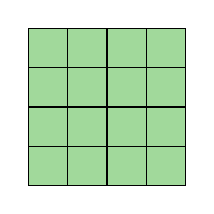
\begin{tikzpicture}[scale=.5]
	\draw[thin, black,fill=green2] (0,0) grid (4,4) rectangle (0,0) ;
	\end{tikzpicture}
	} ;
	\end{scope}
	\begin{scope}
	\node{
	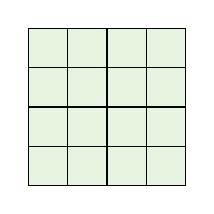
\begin{tikzpicture}[scale=.5]
	\draw[thin, black,fill=green1] (0,0) grid (4,4) rectangle (0,0) ;
	\end{tikzpicture}
	};
	\end{scope}
	% Blue
	\begin{scope}[xshift=4.5cm, yshift=1cm]
	\node{
	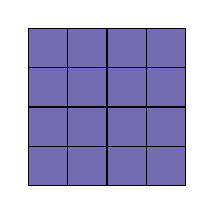
\begin{tikzpicture}[scale=.5]
	\draw[thin, black,fill=blue3] (0,0) grid (4,4) rectangle (0,0) ;
	\end{tikzpicture}
	};
	\end{scope}
	\begin{scope}[xshift=4cm, yshift=.5cm]
	\node[](blue){
	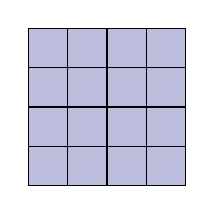
\begin{tikzpicture}[scale=.5]
	\draw[thin, black,fill=blue2] (0,0) grid (4,4) rectangle (0,0) ;
	\end{tikzpicture}
	};
	\end{scope}
	\begin{scope}[xshift=3.5cm]
	\node{
	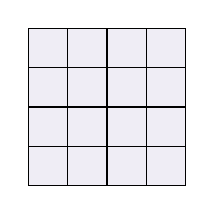
\begin{tikzpicture}[scale=.5]
	\draw[thin, black,fill=blue1] (0,0) grid (4,4) rectangle (0,0) ;
	\end{tikzpicture}
	};
	\end{scope}
\end{tikzpicture}}
\caption{\em Tensor representation of two longitudinal networks as stacked sociomatrices.  One attribute is shown in
purple (e.g., Verbal Cooperation), and the other (e.g., Verbal Cooperation) in green. More recent time slices are shown in darker hues. \label{fig:tensor}}
\end{figure}


\section*{Tensor Methods for Analyzing International Event Count Data}

\section*{Basic Results}

\section*{What Can We Learn?}

\section*{Summary}



\bibliographystyle{apsr}  %asa
\bibliography{/Users/mdw/git/whistle/master}
\newpage
\end{document}  \bye

playground

